\documentclass[final]{beamer}
\usefonttheme[onlymath]{serif}
\usepackage{subfig}
\usepackage{xcolor}
\usepackage[utf8]{inputenc}
\usetheme{SUPoster}
\usepackage{multicol}
\usepackage{diagbox}
\usepackage{tabularx}
\usepackage{booktabs}
\usepackage{todonotes}

%\usepackage[demo]{graphicx}
\usepackage{caption}
\usepackage{subcaption}


\usepackage[orientation=landscape,size=a1,scale=1.6]{beamerposter}

\captionsetup[figure]{labelformat=empty}% redefines the caption setup of the figures environment in the beamer class.
%\captionsetup[subfigure]{labelformat=empty}
\usepackage[absolute,overlay]{textpos}
\setlength{\TPHorizModule}{1cm}
\setlength{\TPVertModule}{1cm}


\usepackage{lmodern} % needed to make math mode fonts scale properly
\usepackage{url}
\usepackage{graphics}
\usepackage{bold-extra}
\usepackage{movie15}
\usepackage{caption}

\usepackage{enumitem}
% \setitemize[1]{label=$\blacktriangleright$}
% \setlist[itemize,1]{label=$\blacktriangleright$}

\setlist[itemize]{label=\usebeamerfont*{itemize item}%
  \usebeamercolor[fg]{itemize item}
  \usebeamertemplate{itemize item},
  leftmargin=1em}

% next line is necessary to make beamer and enumitem play nicely together (see http://tex.stackexchange.com/questions/45921/make-enumerate-have-beamer-themes-when-using-enumitem/45950#45950)
\setlist[enumerate]{leftmargin=2.2em,%
label=\protect\usebeamerfont{enumerate item}%
    \protect\usebeamercolor[fg]{enumerate item}%
    \insertenumlabel. }

%% DOCUMENT DATA

\title{A Formal Methods Approach Towards Deep Learning Interpretability}

\author{Kriten Kessel, Christopher Lazarus, Javier Sagastuy}
\institute{Stanford University}

\logoleft{\begin{center} \includegraphics[height=4.5cm]{img/SU_Seal_Blk_pos}\end{center}}
\logoright{\begin{center} \includegraphics[height=4.5cm]{img/icme_logo_trans} \end{center}}
\footer{CS 236: Deep Generative Models $|$ Fall 2019 \hspace{38cm} \{\texttt{kkessel, clazarus, jvrsgsty}\}\texttt{@stanford.edu} }
%\date{}

\begin{document}


\definecolor{almostWhite}{RGB}{240,240,240}
\definecolor{lightGray}{RGB}{220,220,220}
\definecolor{tbllinecolor}{RGB}{200,200,200}
\beamertemplateshadingbackground{lightGray}{almostWhite}
\newcommand{\vltbl}{{\color{tbllinecolor}\vrule}}


\begin{frame}[fragile]{}

%%%%%%%%%%%%%%%%%%%%%%%%%%%%%%%%%%%%%%%%%%%%%%%%%%%%%%%%%%%%%%%%%%%%
% IMPORTANT:
%   Here is where you define your poster's layout params (widths and
%   vertical positions).
%   Feel free to add/remove more, to make your layout fit your needs
%
%   All dimensions are in cm (I think).
%%%%%%%%%%%%%%%%%%%%%%%%%%%%%%%%%%%%%%%%%%%%%%%%%%%%%%%%%%%%%%%%%%%%

% centralize columns layout
\newcommand{\vstart}{58} % where the top row start vertically
\newcommand{\vstartCols}{8} % where the columns start vertically
\newcommand{\fullwidth}{81}  % this is the key to the values below
\newcommand{\colwidth}{26.5}

\newcommand{\firstcolpos}{1}
\newcommand{\secondcolpos}{28.75}
\newcommand{\thirdcolpos}{56.5}
\newcommand{\bottomblockstart}{108.5}


% this will add some padding to the blocks, to avoid text reaching
% the border (looks bad)
\newenvironment{paddedBlock}[2][0.95\linewidth]
    {\begin{block}{#2}\begin{minipage}{#1}}
    {\end{minipage}\end{block}}

%%%%%%%%%%%%%%%%%%%%%%%%%%%%%%%%%%%%%%%%%%%%%%%%%%%%%%%%%%%%%%%%%%%%
% And now ... the content
%%%%%%%%%%%%%%%%%%%%%%%%%%%%%%%%%%%%%%%%%%%%%%%%%%%%%%%%%%%%%%%%%%%%

%%%%%%%%%%%%%%%%%%%%%%%%%
%%%%%%%%%%%%%%%%%%%%%%%%%
%% LEFT COLUMN
%%%%%%%%%%%%%%%%%%%%%%%%%
%%%%%%%%%%%%%%%%%%%%%%%%%
\begin{textblock}{\colwidth}(\firstcolpos,\vstartCols)

\begin{paddedBlock}{Summary}
Deep Neural Networks are very useful at classifying tasks but their intrinsic complexity makes it really hard to explain the reasoning behind a classification outcome. In recent work [2], statistical methods were introduced to help assess the influence of human intelligible concepts in classification outcomes.
We aim to asses and extend such methods by leveraging formal methods for Neural Network verification.
\begin{itemize}
\item \textbf{Problem:} Why did the network classify image $\mathcal{i}$ with label $k$?
\item \textbf{Solution:} Come up with classes TCAV etc bla bla? or more like we tried to test the TCAV method??
\item \textbf{Preliminary Results:} nothing nothing nothing.
\end{itemize}
\end{paddedBlock}

\begin{paddedBlock}{Talk about TCAV ?}
\underline{Input}:
\begin{itemize}
\item adjacency matrices $A_L$ and $A_U$ for the two sets of nodes;
\item features vectors $X_L$ and $X_U$;
\item labels $y_L$
\end{itemize}
\begin{figure}
    \centering
    %\missingfigure[width=0.5\textwidth]{2 graphs fig}
    %\missingfigure{figure with the two graphs (one labeled and one not) goes here}
    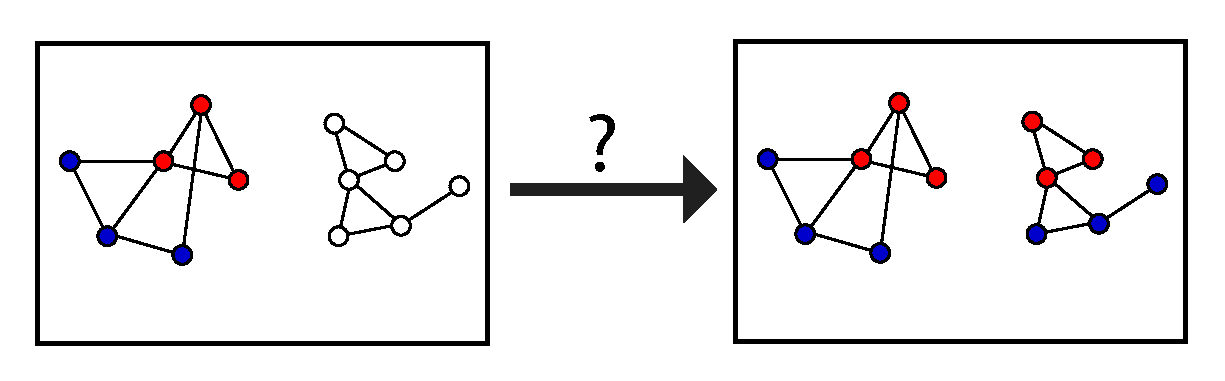
\includegraphics[width=0.90\textwidth]{img/graph_prob.pdf}
    %\caption{Caption}
    \label{fig:coins}
\end{figure}
\underline{Output}:
\begin{itemize}
	\item predictions for the unlabelled nodes $\hat{y}_L$
\end{itemize}
%\vspace{-5mm}
\end{paddedBlock}

\begin{paddedBlock}{Neural Network Verification}
\texttt{GCN} [1] for node classification: $\hat{y} = h(Ah(AXW_1)W_2)$
\begin{figure}
    \centering
    %\missingfigure[width=0.5\textwidth]{2 graphs fig}
    %\missingfigure{architecture of the baseline model}
    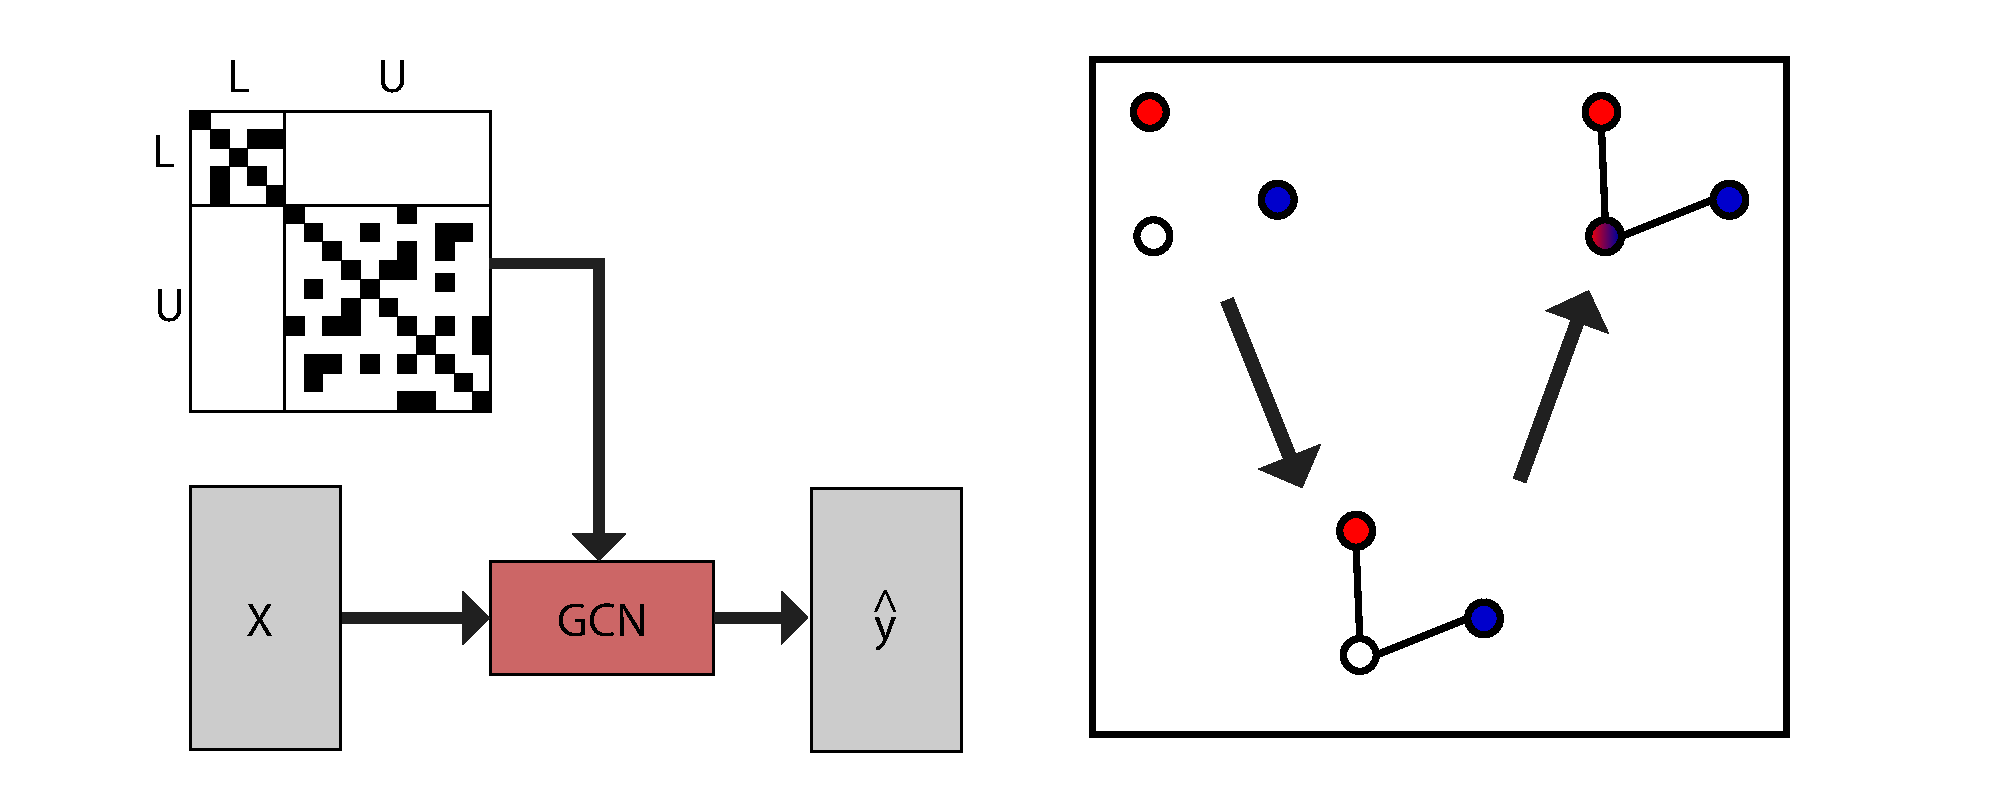
\includegraphics[width=.8\textwidth]{img/model_small.pdf}
    %\caption{Caption}
    \label{fig:small}
\end{figure}
\end{paddedBlock}
\end{textblock}

%%%%%%%%%%%%%%%%%%%%%%%%%
%%%%%%%%%%%%%%%%%%%%%%%%%
%% RIGHT COLUMN
%%%%%%%%%%%%%%%%%%%%%%%%%
%%%%%%%%%%%%%%%%%%%%%%%%%
\begin{textblock}{\colwidth}(\secondcolpos,\vstartCols)
\begin{paddedBlock}{Approach: TCAV + Verification}
%\vspace{8mm}

\alert{Data bla bla}
  \begin{itemize}
    \item talk about data
  \end{itemize}

\begin{figure}%
    \centering
    \subfloat[label 1]{{\includegraphics[width=5cm]{img/mnist_bw.png} }}%
    \qquad
    \subfloat[label 2]{{\includegraphics[width=5cm]{img/mnist_color.png} }}%
    \caption{2 Figures side by side}%
    \label{fig:example}%
\end{figure}

\begin{figure}
    \centering
    %\missingfigure[width=0.5\textwidth]{2 graphs fig}
    %\missingfigure{Hallucigraph architecture sketch}
    \includegraphics[width=.2\textwidth]{img/cav_viz}
    %\caption{Caption}
    \label{fig:big}
\end{figure}

%\vspace{8mm}

\alert{Maybe talk about classe sand support vector}
LALALALALAL

\begin{figure}%
    \centering
    \subfloat[label 1]{{\includegraphics[width=.4\textwidth, backgroundcolor=white]{img/data_distr_balanced_test_new2} }}%
    \qquad
    \subfloat[label 2]{{\includegraphics[width=.4\textwidth]{img/data_distr_blue2_test_new2} }}%
    \caption{2 Figures side by side}%
    \label{fig:example}%
\end{figure}


\begin{align*}
\mathcal{L}_{LP}=&-\mathbb{E}_{Z\sim q(Z|A,X)}[A_{ij}\mathrm{log}\tilde{A}_{ij}+(1-A_{ij})\mathrm{log}(1-\tilde{A}_{i,j})]\\
&+\mathrm{KL}(q(Z|A,X)||p(Z)).
\end{align*}
%\vspace{-8mm}

%\vspace{8mm}
\alert{2. Edge hallucination}
  produces $\hat{A}$:
  \begin{itemize}
    \item top$K$ ($K$ hyper-parameter)
    \item sampling using gumbel softmax [4] trick (allows gradients to flow)
  \end{itemize}
\alert{3. Node classification}
\begin{itemize}
	\item $\hat{y} = \mathrm{GCN}(\hat{A}, X)$
\end{itemize}

\end{paddedBlock}
%\vspace{3mm}
\end{textblock}


\begin{textblock}{\colwidth}(\thirdcolpos,\vstartCols)

%\begin{paddedBlock}

%\
%$\hat{y}=\mathrm{GCN}(\hat{A}, X)$

%\end{paddedBlock}

\begin{paddedBlock}{Results}
%\vspace{8mm}

\alert{Need to talk about significant CAVs}
Then talk about the avenues and boulevards.

\begin{figure}
    \centering
    %\missingfigure[width=0.5\textwidth]{2 graphs fig}
    %\missingfigure{Hallucigraph architecture sketch}
    \includegraphics[width=.8\textwidth]{img/scree_plot}
    %\caption{Caption}
    \label{fig:big}
\end{figure}

%\vspace{8mm}
\alert{Node classification results}

\begin{table}
\centering
\begin{tabular}{lcccc}
\hline

\textbf{model} &  \textbf{balanced} &   \textbf{blue 2} &    \textbf{red 2} &  \textbf{green 2} \\ \hline 
\texttt{balanced\_5x50} &    $0.942$ &  $0.942$ &  $0.941$ &  $0.944$ \\
\texttt{blue2\_5x50} &    $0.780$ &  $0.952$ &  $0.682$ &  $0.689$ \\
\texttt{balanced\_3x50} &    $0.942$ &  $0.940$ &  $0.942$ &  $0.941$ \\
\texttt{blue2\_3x50} &    $0.724$ &  $0.954$ &  $0.675$ &  $0.684$ \\
\texttt{balanced\_3x20} &    $0.890$ &  $0.890$ &  $0.891$ &  $0.888$ \\
\texttt{blue2\_3x20} &    $0.708$ &  $0.923$ &  $0.663$ &  $0.672$ \\
\hline

\end{tabular}
\end{table}



\begin{itemize}
  \item Try to salvage somethibg
  \item Nothing worked : )
\end{itemize}

\end{paddedBlock}


\begin{paddedBlock}{References}
\footnotesize{[1] G. Katz, C. Barrett, D. L. Dill, K. Julian, and M. J. Kochenderfer. Reluplex: An efficient smt solver for verifying deep neural networks. In International Conference on Computer Aided Verification, pages 97–117. Springer, 2017}

\footnotesize{[2] B. Kim, M. Wattenberg, J. Gilmer, C. J. Cai, J. Wexler, F. B. Viegas, and R. Sayres. Interpretability beyond feature attribution: Quantitative testing with concept activation vectors (tcav). In ICML, 2018}

\footnotesize{[3] Y. LeCun, C. Cortes, and C. Burges. Mnist handwritten digit database. AT&T Labs [Online]. Available: http://yann. lecun. com/exdb/mnist, 2:18, 2010}

\footnotesize{[4] C. Liu, T. Arnon, C. Lazarus, C. Barrett, and M. J. Kochenderfer. Algorithms for verifying deep neural networks. CoRR, abs/1903.06758, 2019}

\end{paddedBlock}
\end{textblock}


%%%%%%%%%%%%%%%%%%%%%%%%%
%%%%%%%%%%%%%%%%%%%%%%%%%
%% BOTTOM ROW
%%%%%%%%%%%%%%%%%%%%%%%%%
%%%%%%%%%%%%%%%%%%%%%%%%%

%\begin{textblock}{\fullwidth}(2,\bottomblockstart)
%\begin{paddedBlock}[0.98\linewidth]{Acknowledgements}

%In case you need it, you can do this too

%\end{paddedBlock}
%\end{textblock}

\end{frame}
\end{document}
